What to try next for improving our neural networks?
\begin{itemize}
  \item Getting more training examples
  \item Trying smaller sets of features
  \item Trying additional features
  \item Trying polynomial features
  \item Increasing or decreasing $\lambda$
\end{itemize}

\section{Evaulating a Hypothesis}
A hypothesis may have a low error for training examples but still be inaccurate (because of overfitting). Thus, to evaulate a hypothesis, given a dataset of training examples, we can split up the data into two sets: a training set and a test set. Typically, the training set consists of $70\%$ of your data and the test set is the remaining $30\% $.

\begin{figure}[h]
  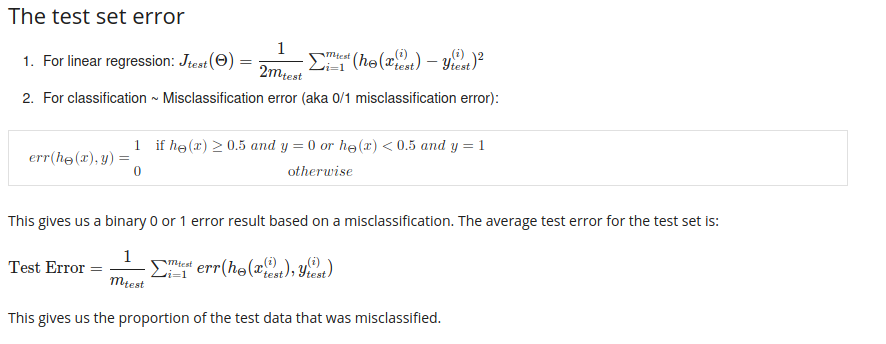
\includegraphics[scale=0.5]{testerror.png}
\end{figure}

\subsection{Model Selection}
  Just because a learning algorithm fits a training set well, that does not mean it is a good hypothesis. It could over fit and as a result your predictions on the test set would be poor.
  \\\\
  Given many models with different polynomial degrees, we can use a systematic approach to identify the 'best' function. In order to choose the model of your hypothesis, you can test each degree of polynomial and look at the error result.
  \\\\
  We usually break down out dataset into three sets:
  \begin{itemize}
    \item Training set: $60\%$
    \item Cross validation set: $20\%$
    \item Test set: $20\%$
  \end{itemize}


  Now to improve our training:
  \begin{enumerate}
    \item Optimize the parameters in $\theta$ using training set.
    \item Find the polynomial degree $d$ with the least error usign the cross validation set.
    \item Estimate the generalization error using the test set with $J_{test}(\Theta^{(d)})$ (d = $\theta$ from polynomial with lower error)
  \end{enumerate}

\section{Bias vs. Variance}
  \textbf{High bias (underfitting)}: both $J_train(\theta)$ and $J_{CV}(\theta)$ will be high and also similar.
  \\\\
  \textbf{High variance (overfitting)}: $J_train(\theta)$ will be low but $J_{CV}(\theta)$.\\

  \begin{figure}[h]
    \centering
    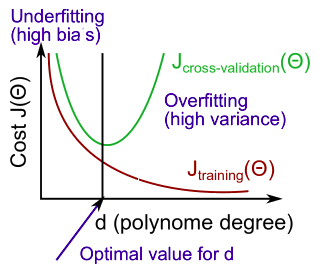
\includegraphics[scale=0.5]{biasVariance.png}
  \end{figure}

  \subsection{Regularization}

    \begin{figure}[h]
      \centering
      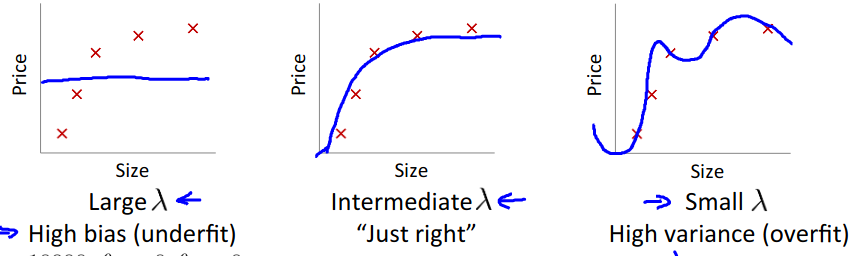
\includegraphics[scale=0.5]{lambda.png}
      \caption{Fitting of data with $\lambda$}
    \end{figure}

    In the figure above, we see that as $\lambda$ increases, our fit becomes more rigid. On the other hand, as $\lambda$ approaches 0, we tend to over overfit the data. So how do we choose our parameter $\lambda$ to get it 'just right' ?

    \begin{enumerate}
      \item Create a list of lambdas.
      \item Iterate through the $\lambda s$ and for each, go throught all the models to learn some $\theta$
      \item Compute the cross validation error.
      \item Select the best combo of $\theta \& \lambda$.
    \end{enumerate}    

  \subsection{Learning Curves}
    \begin{figure}[h]
      \centering
      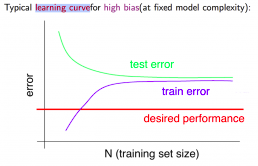
\includegraphics[scale=0.7]{learnbias.png}
      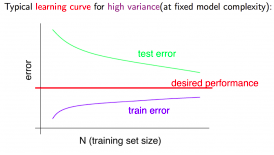
\includegraphics[scale=0.75]{learnvariance.png}
    \end{figure}    
  
